\subsection{Interviews}

\subsection{Literature studies}

\subsection{Workshop}
\subsubsection{Planning}
As part of the pre-study, it was planned from the start of the project to host a workshop. A workshop is an interactive session in which participants work together on solving issues through discussion and brainstorming\cite{workshop}. 

A subgroup of the project members were responsible for planning and hosting the workshop. The planning consisted of brainstorming sessions and a consulting session with the project owner for advice on how to manage a workshop. An important question that was discussed in the brainstorming process was what the actual purpose of the workshop should be. It was decided on holding the workshop with the second out of two purposes:

\begin{list_type}  
    \item Try out game mechanics on the participants to see which mechanics should be included in the product.
    \item Find out from the participants what features the product should have and mockups of the suggested system. 
\end{list_type}

To elicit information in the workshop in accordance to the purpose of the workshop, three workshop scenarios were designed. The idea behind the scenarios is to have the participants discuss freely on certain issues that are relevant to the product. Short description of the three scenarios (for full information see \ref{chapter:workshop}):

\begin{list_type}  
    \item \textbf{Scenario 1:} Put the participants in the role of a student having to complete complete cumbersome programming assignments, think of a system that would make this more appealing.
    \item \textbf{Scenario 2:} Put the participants in the role of a teacher which years later holds the same course. Further develop and/or limit the system.
    \item \textbf{Scenario 3:} User-interface mockups of the system.
\end{list_type}
    
\subsubsection{Hosting}
Invitations were sent to students, teachers and employees at the University Pedagogy Centre, all from Luleå University of Technology. There were 12 participants in total, five of which were moderators. The participants were randomly split into two groups. They received print-outs of the scenarios and had limited time to discuss and write down ideas on post-it notes and white-boards, which would later be presented.

\begin{figure}[H]
\centering
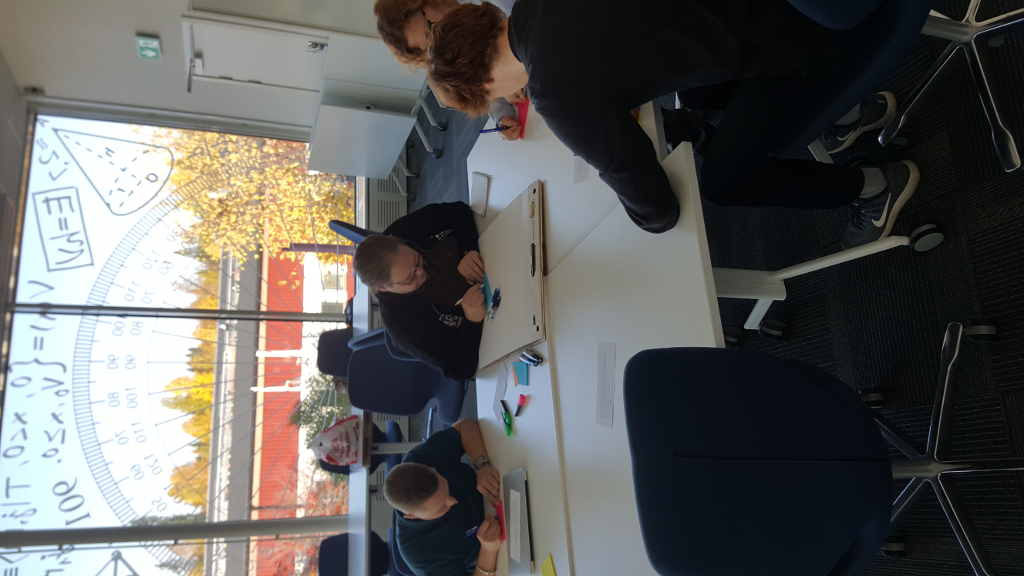
\includegraphics[width=0.8\textwidth]{img/gppinpictures/workshop1_resized.jpg}
\caption{Workshop in action: 1}
\label{fig:workshop1}
\end{figure}

\begin{figure}[H]
\centering
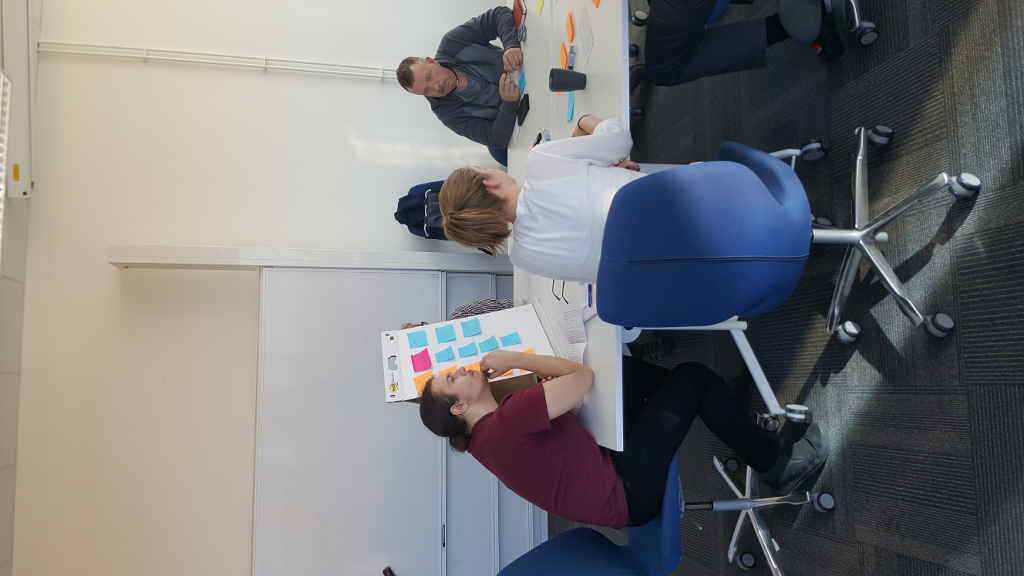
\includegraphics[width=0.8\textwidth]{img/gppinpictures/workshop2_resized.jpg}
\caption{Workshop in action: 2}
\label{fig:workshop2}
\end{figure}

\begin{figure}[H]
\centering
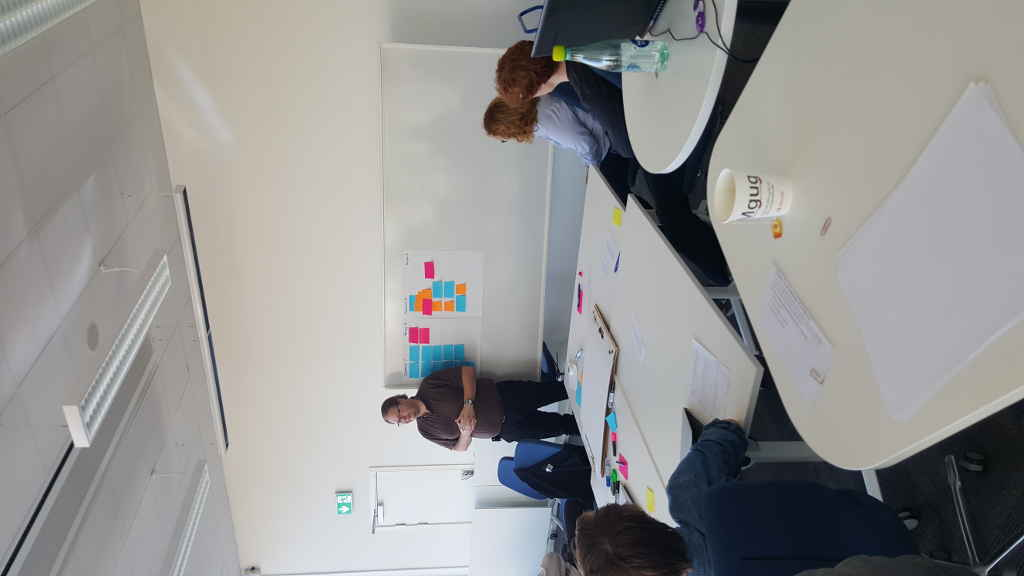
\includegraphics[width=0.8\textwidth]{img/gppinpictures/workshop3_resized.jpg}
\caption{Workshop in action: 3}
\label{fig:workshop3}
\end{figure}

\subsubsection{Results}
Summarized results from the workshop:

\begin{itemize}
    \item Gamification elements will motivate students to perform the assignments.
    \item Social support, encourage students to cheer for one-another through collaboration.
    \item Anonymous questions so students doesn't have to be afraid to ask questions. Should generate statistics for the teacher.
    \item More direct contact between teachers and students, live-chat.
    \item Fast feedback for students when doing assignments. 
    \item Personality tests to customize gamification elements and/or UI.
    \item Students correct assignments completed by other students, and create assignments for one another.
    \item An internal knowledge-bank for the system, similar to \href{https://stackoverflow.com/}{Stackoverflow}, where students can find help with certain courses and/or assignments.
\end{itemize}

\begin{figure}[H]
\centering
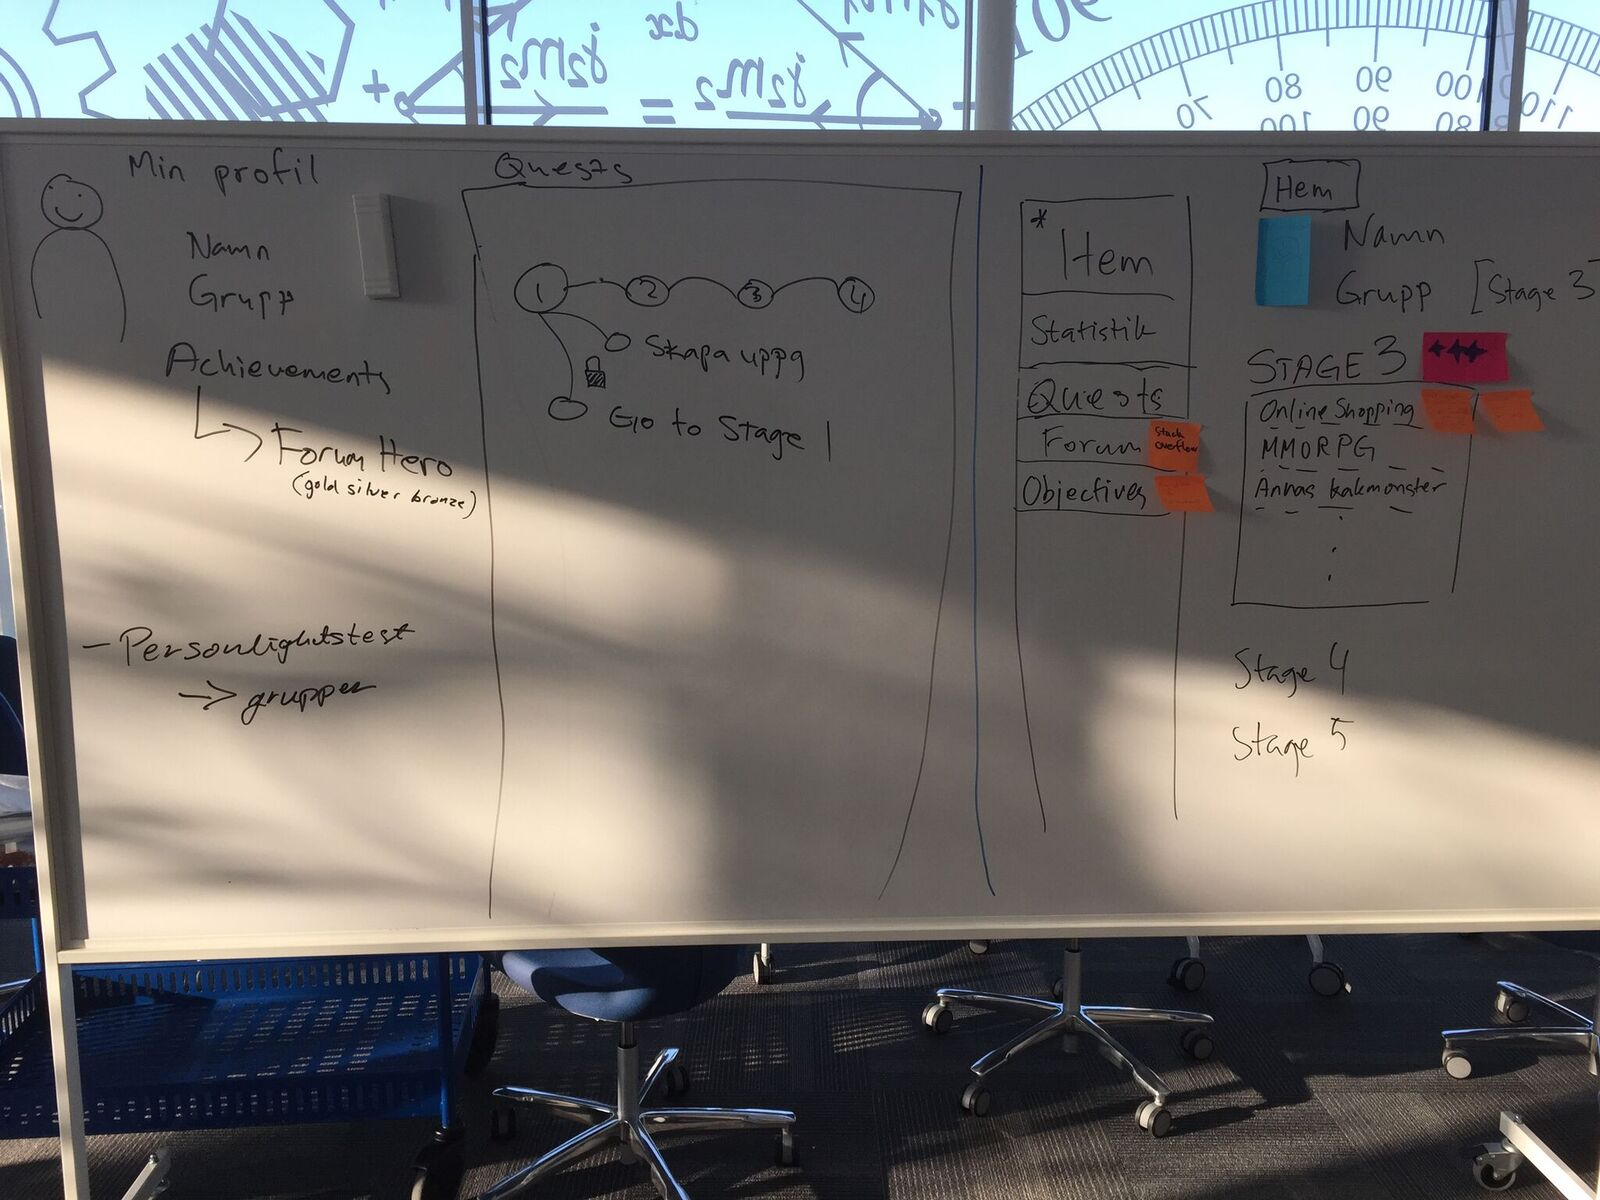
\includegraphics[width=0.8\textwidth]{img/gppinpictures/Grupp2_Workshop_mockup.jpg}
\caption{Workshop in action: 4}
\label{fig:workshop4}
\end{figure}
